\section{The \qevis{} System}\label{sec:qevis}
The architecture of \qevis{} is illustrated in \autoref{fig:arch}.
%When a query is executed in distributed query system, the data collection module collects the query execution logs and stores them in the backend database.
%These data are fed into the visualization module to generate the user interface. 
In this section, we first introduce the system architecture in \autoref{sec:architecture}. Then we discuss data model of \qevis{} in \autoref{sec:data} and elaborate on the visualization designs 
%to support multi-grained exploration 
in \autoref{sec:design}.


\begin{figure}[t]
	\centering
	\includegraphics[width=0.42\textwidth]{figures/framework/Systemframework.pdf}
	\vspace{-3mm}
	\caption{ 
		\qevis{} system includes three modules: (1) data collection module, (2) data analysis module, and (3) visualization and interaction module
	}
	\label{fig:arch}
	\vspace{-3mm}
\end{figure}


\subsection{System Architecture} \label{sec:architecture}
We developed a prototype of \qevis{} and kept improving it according to user feedback. 
\autoref{fig:arch} illustrates the final system architecture and analysis pipeline of \qevis{}. 
The system consists of three modules for (1) data collection, (2) data analysis, and (3) visualization and interaction. 	
When users run a query, the data collection module collects and processes incoming query execution logs with the stream log engine.
Specifically, it persists the basic information and passes logs to the database until execution status indicators (i.e.,  \textit{Pause}, \textit{Terminate}, \textit{Complete}, \textit{Timeout}) are detected.  
To monitor query execution at run time, the stream log engine redirects processed logs to the frontend for visualization.
In the meantime, the logs are stored in a database to enable in-depth analysis of completed queries.
The data analysis module reads data from the database and calculates anomaly scores. 
The visualization and interaction module displays the query execution process and provides rich interactions to support interactive exploration.


\subsection{Data Model}\label{sec:data}
As introduced in \autoref{sec:qryprocessing}, a query is converted to a DAG of Map/Reducer jobs during query execution. We denote the DAG as $G(J,R)$, where $J$ is the node set, and each node is a Map or Reducer job in the logic execution plan; $R$ is the edge set, which models the dependencies among the jobs.
For each atomic task, we divide its execution process into three phases 
%according to the logs
: (1) input, (2) processing, and (3) output, for fine-grained analysis. 
We use $t_{exe}=\{(t_s^i, t_e^i), (t_s^p,  t_e^p), (t_s^o, t_e^o) \}$ to denote the start time and end time of each phase in task $t$.
Thus, the data model of task $t$ is a tuple $\langle t_s, t_e, t_j, t_m, t_{exe} \rangle$, which are the task's start time, end time, job identifier, machine identifier and the execution phases, respectively. The data model of each job is a tuple $\langle j_s, j_e \rangle$, which are the job's start time and end time, respectively.
A job has many tasks, for job $x$, its start time $j_s$ is defined as the earliest start time of all its tasks, i.e., $j_s = \min \{ t_s | t_j = x \}$, and its end time $j_e$ is the latest end time of all its tasks, i.e., $j_e = \max \{ t_e | t_j = x \}$.
With the data model above, the original job DAG is augmented to a temporal DAG (TDAG), which contains start/end time for each job and is key to query execution analysis.





\subsection{Visualization Designs in \qevis{}}\label{sec:design}


With the design tasks of \qevis{} in mind, we present our proposed techniques to achieve that.
Specifically, \autoref{fig:teaser} illustrates the user interface of \qevis{}.
With a selected query from the \vtitle{query list} (\autoref{fig:teaser}(a)), \vtitle{job view} appears to provide the overview of query execution (\textbf{T1.1}), which is shown as \autoref{fig:teaser}(b). We devise a novel algorithm to generate a timeline-based visualization to show the timing information of jobs and their dependencies, which is elaborated in \autoref{sec:job}.
In \autoref{sec:taskmachinepair}, we provide a \vtitle{performance matrix} to show the anomaly degree of the jobs and machines, which is shown in \autoref{fig:teaser}(c). \vtitle{Performance matrix} helps users quickly narrow down to the jobs and machines that are \qm{worth paying attention to} (\textbf{T2}). 
In \autoref{sec:task}, we design the \vtitle{task view} to support fine-grained task analysis (\textbf{T1.2}), which is shown in \autoref{fig:teaser}(d).
In \autoref{sec:other}, we present the auxiliary views for detailed information (\textbf{T3.1}) and cross-view linkages for interactive exploration (\textbf{T3.2}).

\subsubsection{Job view}\label{sec:job}

\begin{figure}
	\centering
	\small
	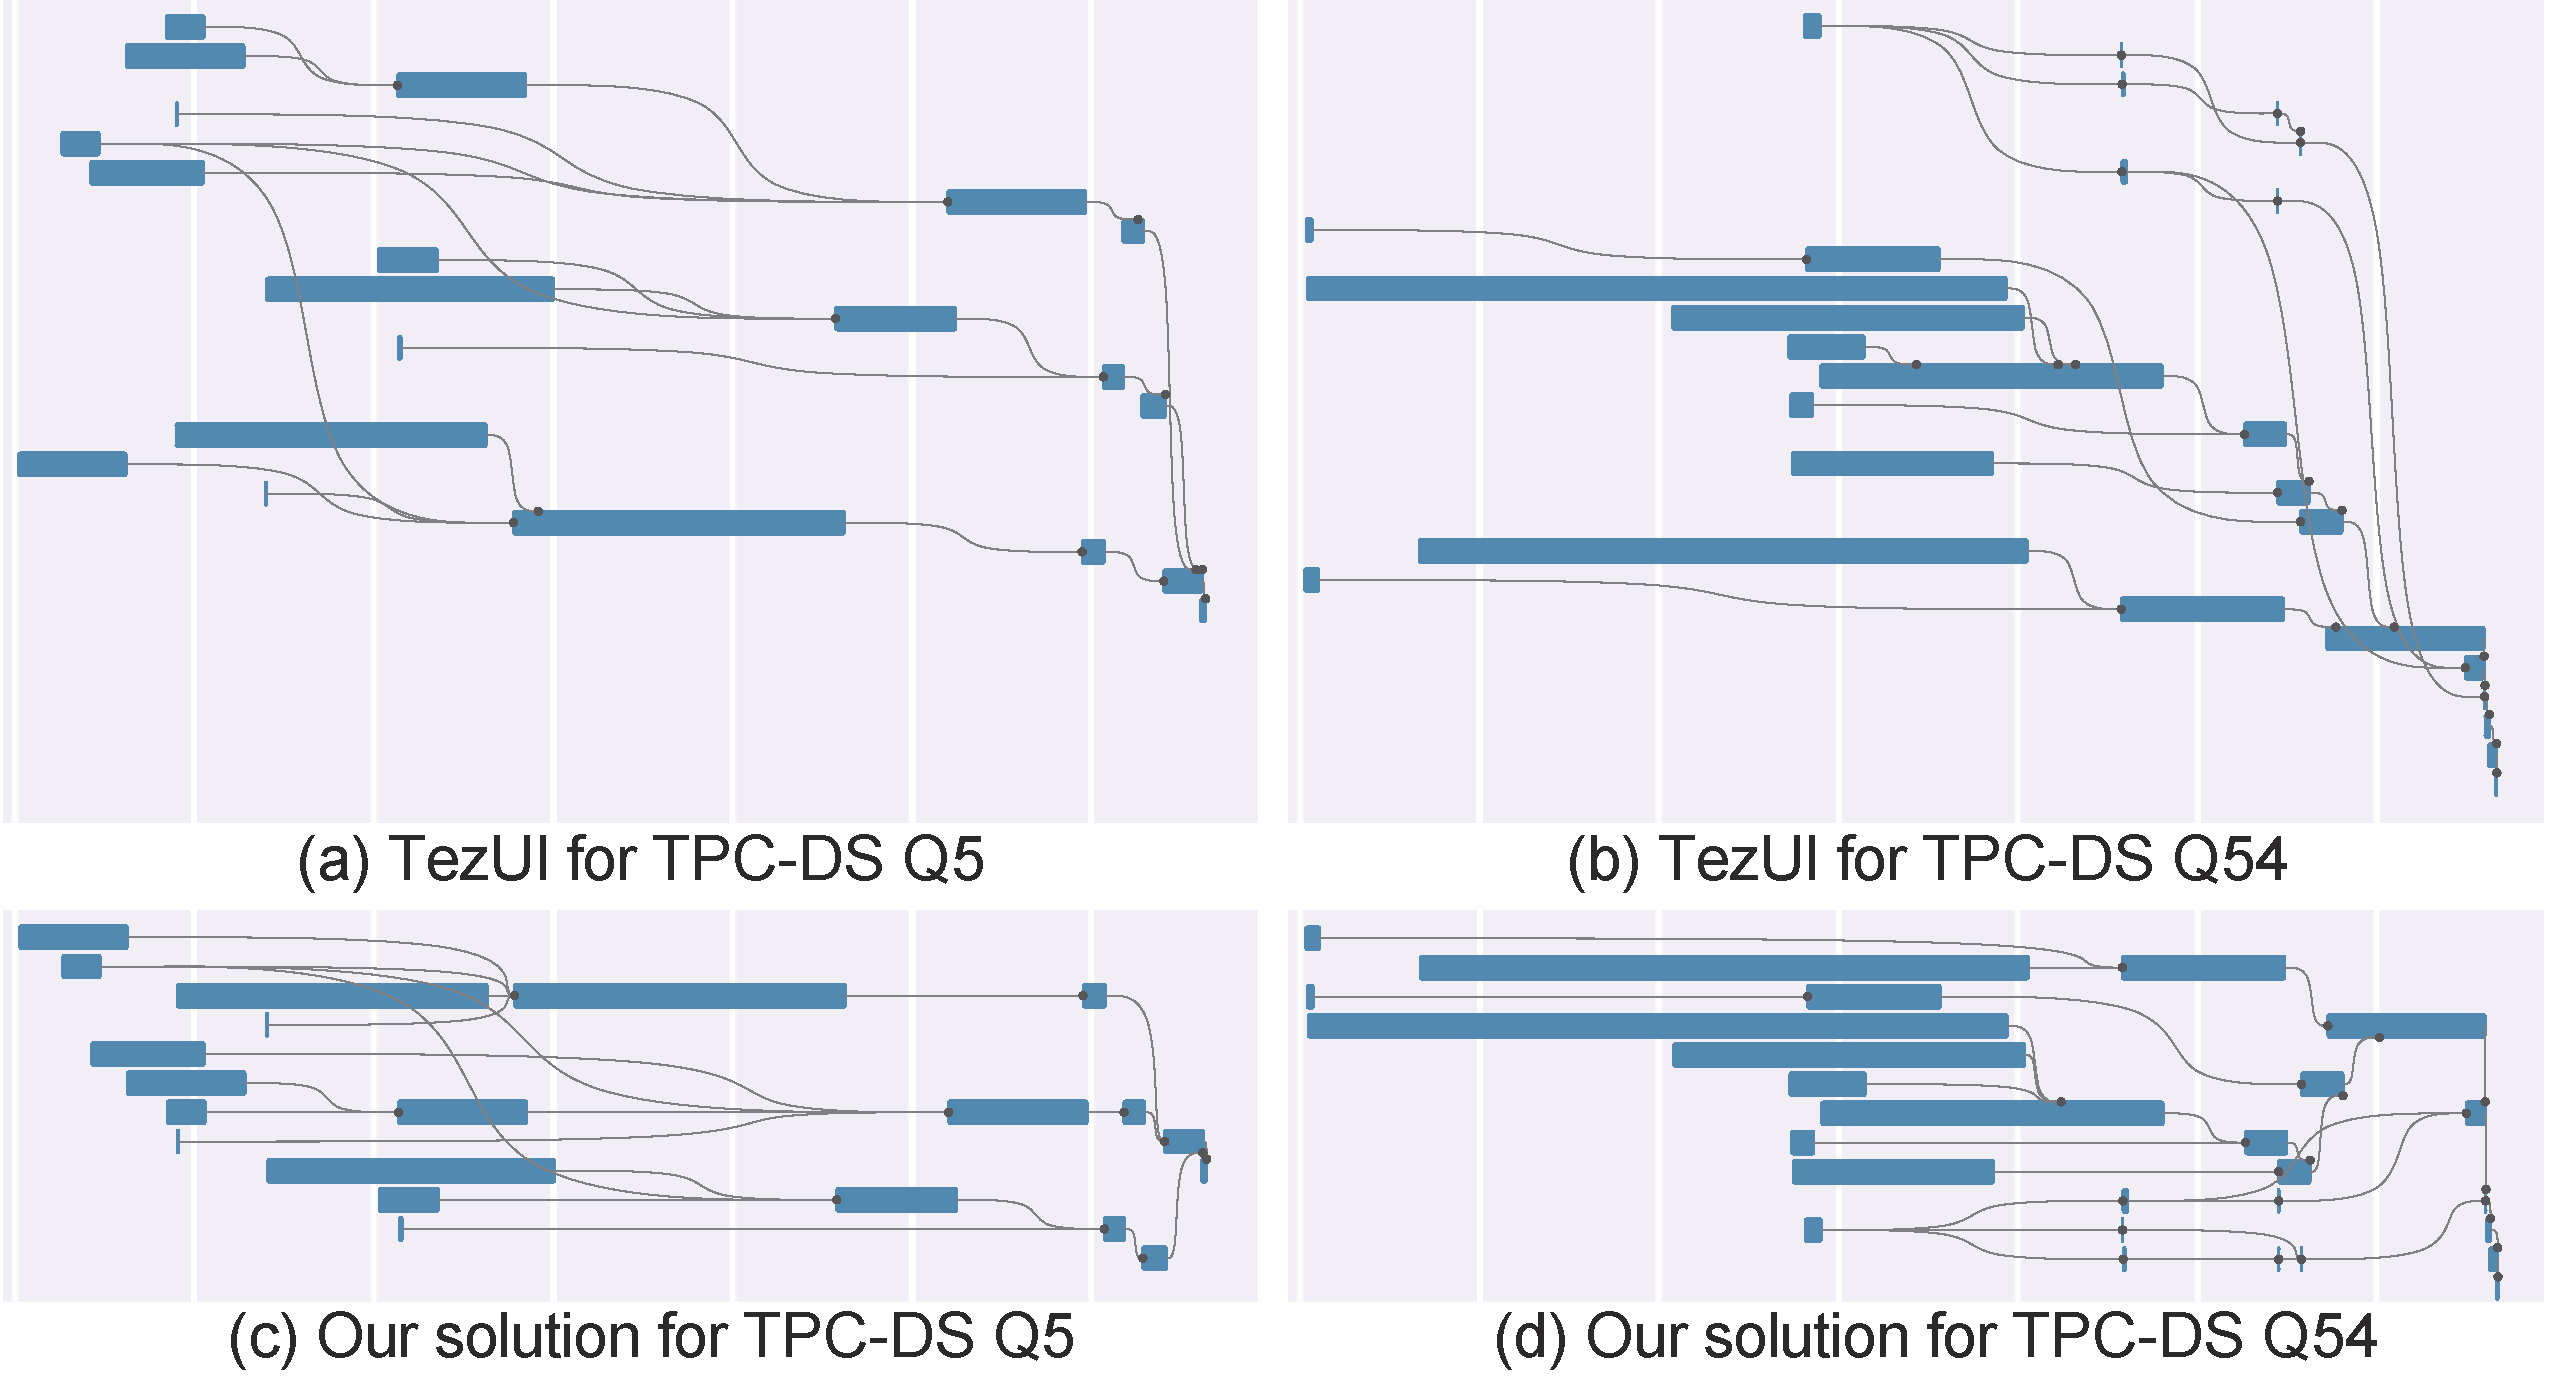
\includegraphics[width=0.44\textwidth]{figures/visualization/exeprogressSDS.pdf}
	\vspace{-3mm}
	\caption{Comparing TDAG layout methods}
	\label{fig:layout}
	\vspace{-3mm}
\end{figure}

\begin{figure}
	\centering
	\small	
	\includegraphics[width=0.42\textwidth]{figures/visualization/TDAG-new-algo.pdf}
	\vspace{-3mm}
	\caption{Workflow of our TDAG layout algorithm}
	\label{fig:layoutmethod}
	\vspace{-5mm}
\end{figure}




To effectively visualize the progress of job execution, it is essential to display the timing information, including start time, end time, and time usage, as well as the dependencies among jobs in the query logical plan (\textbf{T1.1.1} and \textbf{T1.1.3}). This data can be modeled as a DAG enhanced with temporal information (TDAG).
Existing tools (e.g., TezUI and SparkUI) enhance traditional Gantt chart with links to visualize the TDAG. 
This solution is limited because (i) it does not consider the visual clutter caused by the many job dependencies in the execution plan; and (ii) it does not scale to large TDAG as screen space is not utilized efficiently. \autoref{fig:layout} (a) and \autoref{fig:layout}(b) show its visualizations for the TDAG of TPC-DS query 5 and 54, respectively. The edges and nodes are crossed in \autoref{fig:layout}(a) due to complex job dependencies, and there is a large blank space in the left bottom part of \autoref{fig:layout}(b).


To tackle the two challenges, we propose a novel TDAG layout method illustrated in \autoref{fig:layoutmethod}. It includes the following steps:

\squishlist
\item \stitle{Step 1} We first simplify the job DAG, see \autoref{fig:layoutmethod}(a), to a job dependency tree in \autoref{fig:layoutmethod}(b).
In particular, the output of a job can be the input of many jobs (e.g., $\geq 2$ jobs), and we only preserve the edge from a job to its out-neighbor job with the earliest start time.
For example, the output of job $1$ serves as input for jobs $4$ and $6$ but the start time of job $4$ is earlier than job $6$. Thus, we only keep the edge from job $1$ to job $4$ in the simplified job tree in \autoref{fig:layoutmethod}(b).
TDAG simplification is conducted to (i) preserve the starting time order of the jobs, and (ii) keep dependent jobs close to each other to prevent visual clutter.

\item \stitle{Step 2} We then plot a rectangle for each job by using the length of the rectangle to indicate job duration and sort the jobs by their start time, as shown in \autoref{fig:layoutmethod}(c).
This follows human reading habit (i.e., reading from top to bottom) and plots the job starting earlier in a higher position. 

\item \stitle{Step 3} We next adjust the layout of jobs by utilizing the job dependencies in the simplified tree. In particular, we check the jobs the top to bottom. For each job, if its out-neighbor job could be placed in the same row with it (i.e., non-overlapping), we move the out-neighbor to the same row with it, and add an edge between these two jobs. 
For instance, the time duration of job $1$ does not overlap with the time duration of its out-neighbor job $4$, thus we plot jobs $1$ and $4$ in the first row, see \autoref{fig:layoutmethod}(c).

\item \stitle{Step 4}  Last, we refine TDAG layout by (i) adding the other edges in the job DAG, for example, jobs $1$ and $6$ in \autoref{fig:layoutmethod}(e), and (ii) reducing the space by combining the rows that do not overlap, for example, job $3$ and job $5$ are plotted in the same row in \autoref{fig:layoutmethod}(e).
\squishend




%We visualize the TDAG of TPC-DS query 5 and query 54 by our TDAG layout algorithm in \autoref{fig:layout}(c) and (d), respectively. Compared with the visualizations produced by Tez UI \autoref{fig:layout}(a) and (b), our visualizations are obviously better. In particular, visual clutter is significantly reduced in our visualization because we consider the dependencies among the jobs via the simplified tree. Moreover, our visualizations take much smaller screen space because our adjustment considers job dependencies and time duration.    
We visualize the TDAG of TPC-DS query 5 and query 54 by our TDAG layout algorithm in \autoref{fig:layout}(c) and \autoref{fig:layout}(d), respectively. 
\qm{
%	Compared with the visualizations produced by Tez UI \autoref{fig:layout}(a) and (b), our visualizations reduce the visual clutter because we consider the dependencies among the jobs via the simplified tree. Moreover, our visualizations take smaller screen space because our adjustment considers job dependencies and time duration.    
%	Compared with the visualizations produced by Tez UI \autoref{fig:layout}(a) and (b), the visualization generated by our approach have two benefits:1) since our approach considers the topological structure of execution plan, the visualization has less visual clutter because it has few crossing among the links and rectangles; 2) the proposed visualization task smaller screen space because the algorithms considers both job dependencies and time duration. 
	When compared with the visualizations produced by Tez UI \autoref{fig:layout}(a) and \autoref{fig:layout}(b), 
	the visualization generated by our approach offers two advantages: (1) our visualization takes into account the topological structure of the execution plan, resulting in reduced visual clutter as there are fewer crossings among the links and rectangles; (2) our proposed visualization optimizes screen space utilization by considering both dependencies and time duration, allowing for a more efficient visualization.
}


We enhance the \vtitle{job view} with two visual designs (i.e., parallelism and phase mode) to show more information for each job (\textbf{T1.1.2}). 

\sstitle{Parallelism mode} we embed the task parallelism (i.e., number of running tasks) into the job rectangle. Specifically, we use a 1D-heatmap to visualize the number of active tasks over time, as shown in \autoref{fig:teaser}(b). 
A gradient color from white to dark blue encodes the number from one to the maximum number of active tasks for the job. We color the number zero with a special color (e.g., gray) as zero indicates that the execution of the job is suspended and users should pay attention. 

\sstitle{Phase mode} we visualize the percentage of time used by the three phases of each job, as shown in \autoref{fig:teaser}(b1), and use three colors to indicate the three phases.  
This allows users to better understand the jobs, e.g., classifying them into I/O-bounded or compute-bounded jobs.



\subsubsection{Performance matrix}\label{sec:taskmachinepair}
As shown in \autoref{fig:teaser}(c), performance matrix is designed to show the anomaly degree of jobs and machines such that users can narrow down the scope of exploration (\textbf{T2}). 
Existing tools~\cite{elephant, prometheus} propose different scoring schemes for different anomaly types, e.g., data skew and memory overload. This approach is limited as it is difficult to encompass all possible anomalies. We adopt a different approach, which considers the execution statistics of the tasks and quantifies how far they deviate from ideal distributed parallel execution. 
We believe a component is \qm{worth paying attention to} if it deviates far from ideal, and we leave it to the users to determine the specific anomalies by inspecting the views we provided.
In the ideal case, all tasks of a job have a similar workload and run in parallel, which results in similar time usage and high parallelism for these tasks.
On this basis, we propose two novel anomaly scores to analyze the tasks of a job, i.e., \textit{abnormal parallelism score} ($\aps$) and \textit{abnormal duration score} ($\ads{}$).

\begin{figure}
	\centering
	\small
	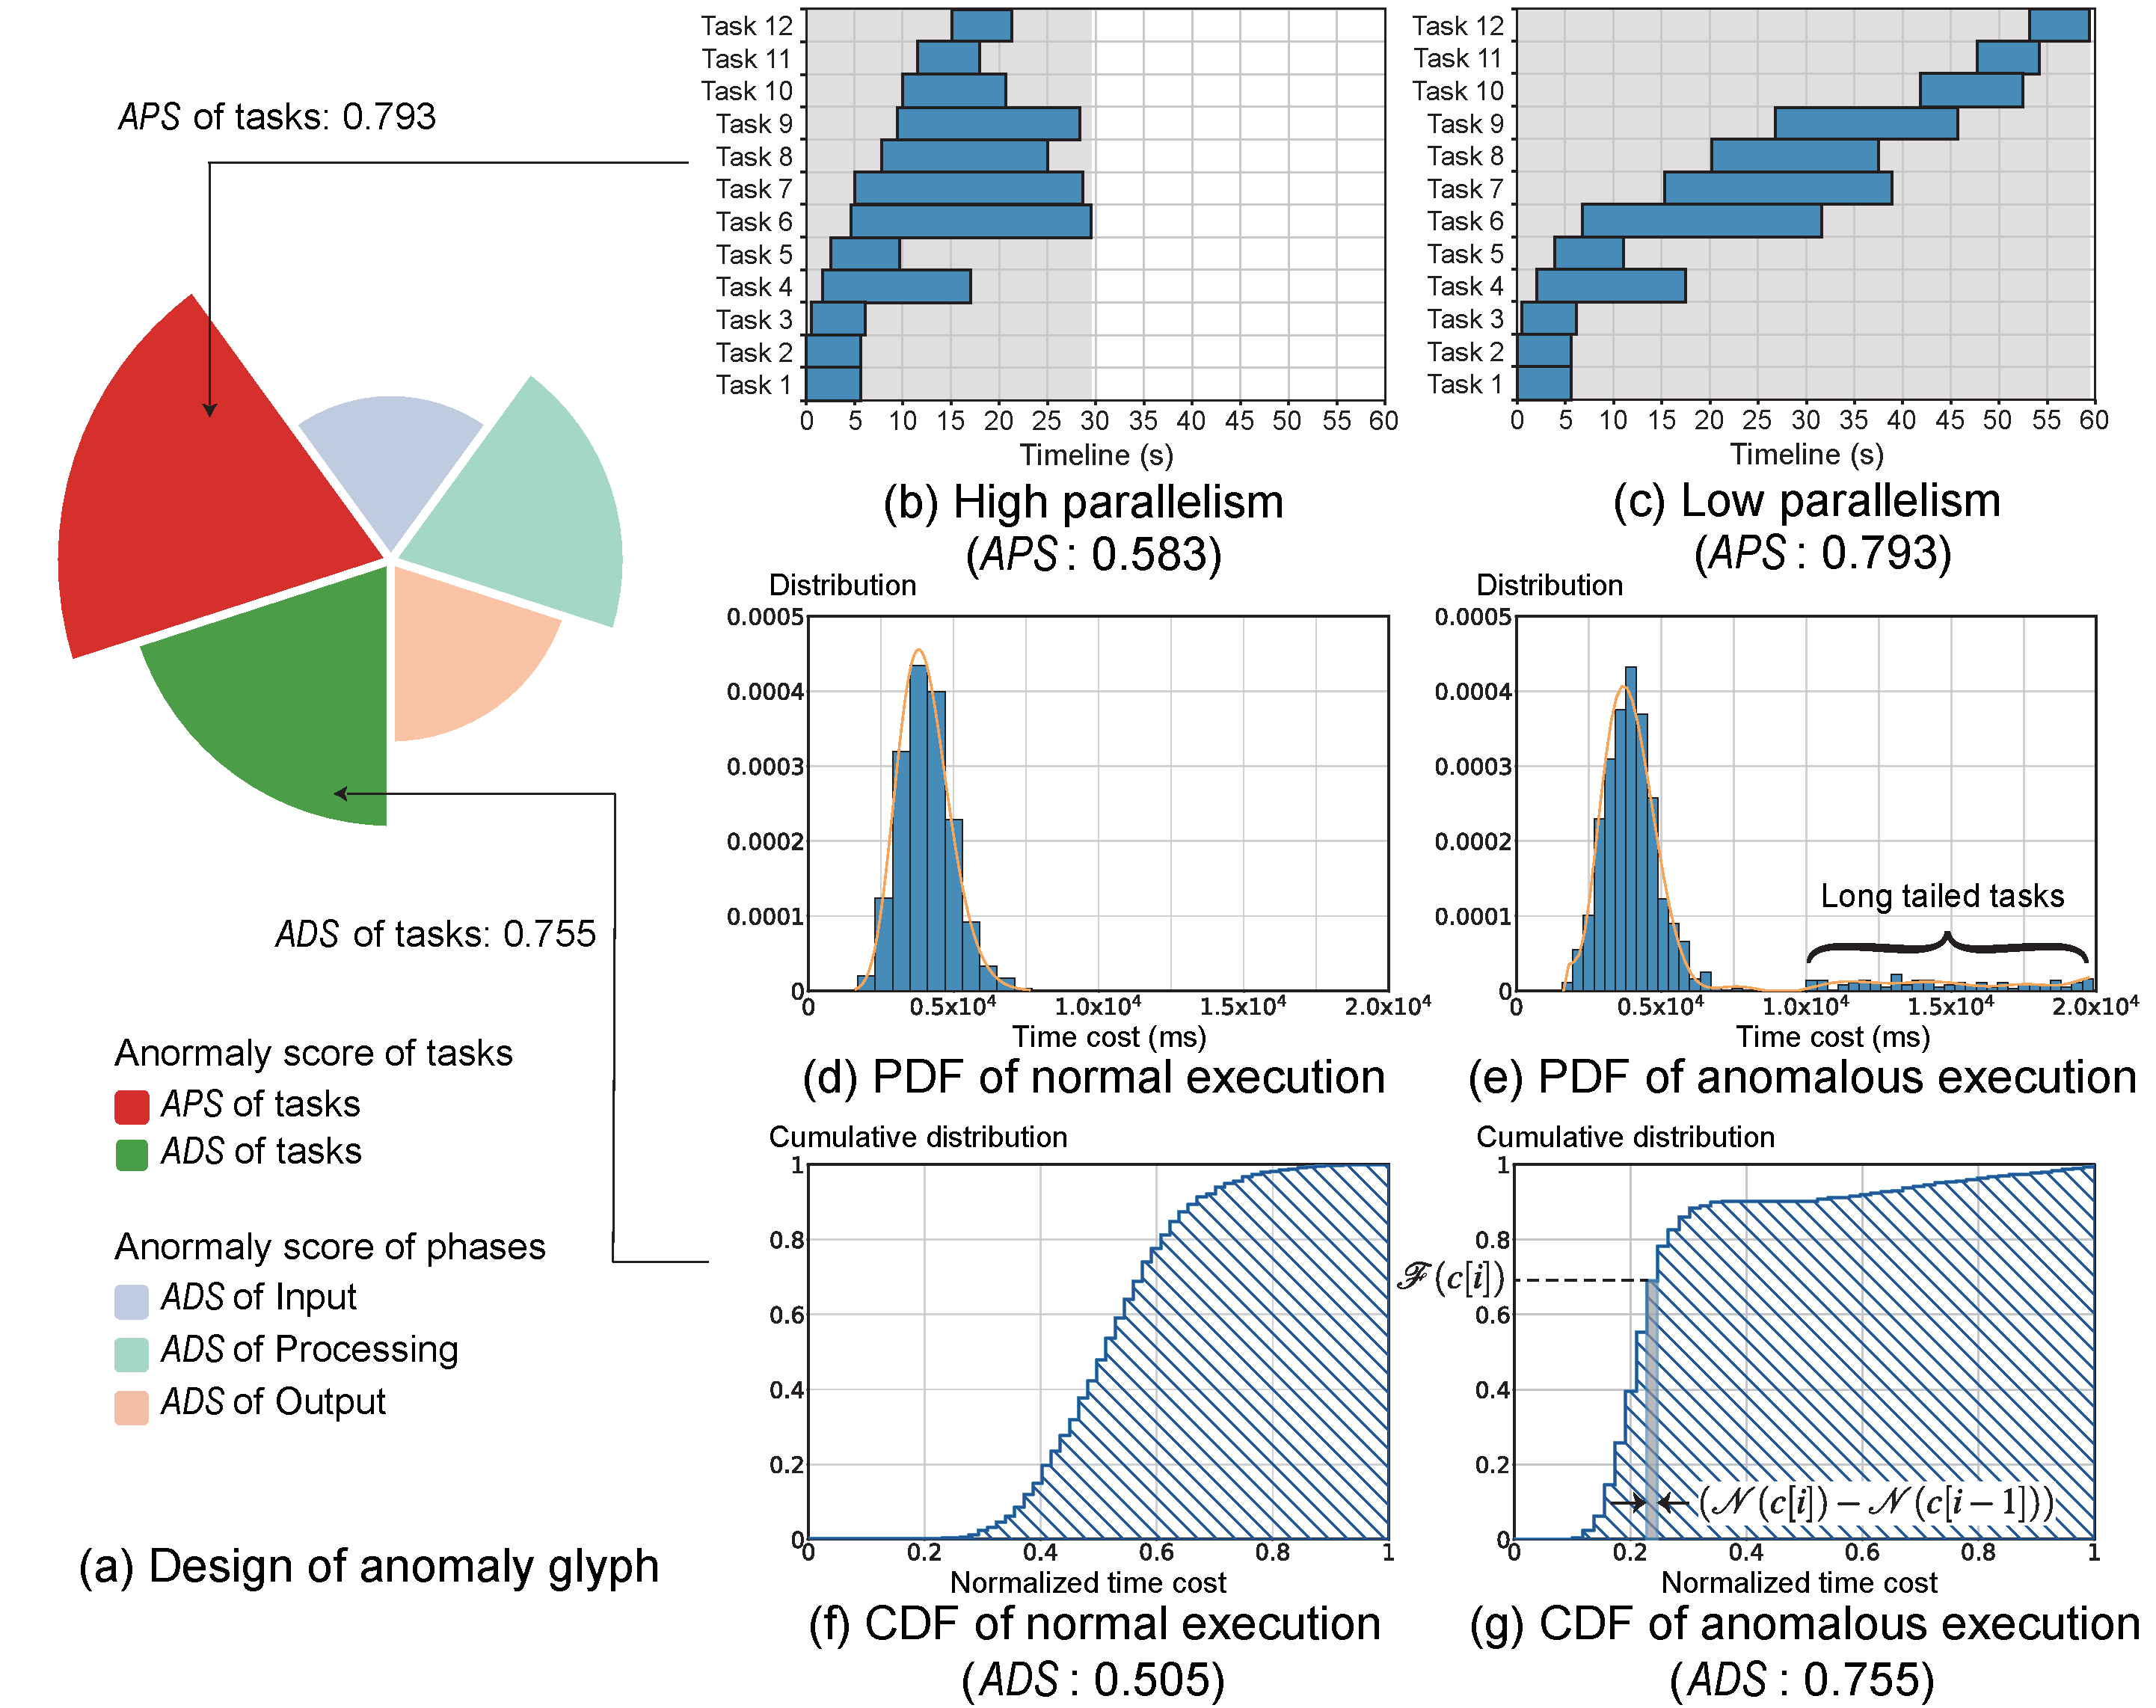
\includegraphics[width=0.42\textwidth]{figures/dataprocess/anomaly_illustration_vis2023.pdf}
	\vspace{-3mm}
	\caption{Illustration of anomaly scores}
	\label{fig:score}
	\vspace{-5mm}
\end{figure}

\stitle{Abnormal parallelism score ($\aps$)} $\aps$ measures how well the tasks of a job are parallelized, \qm{how many jobs share the similar start time and end time.}
%\qm{Parallelism refers to the synchronization of task start and end times.}

For example, the tasks in \autoref{fig:score}(b) are paralleled better than the tasks in \autoref{fig:score}(c) as the tasks are better overlapped in time and more of them run concurrently. Denote the task set of job $j$ as $T_j = \{t_j[1], \cdots, t_j[n]\}$, the $\aps$ of $T_j$ is defined as:
$$\aps(T_j) = 1 - \frac{\sum_{i^=1}^{n} (t_j[i]_e - t_j[i]_s)}{n \times (j_e - j_s)}.$$
Intuitively, the second term of $\aps$ measures the ratio between the area of all tasks (the bars in \autoref{fig:score}(b) and \autoref{fig:score}(c)) over the area of the job rectangle (the gray area in \autoref{fig:score}(b) and \autoref{fig:score}(c)). If all tasks have the same time usage and run concurrently, $\aps$ will be 0, and thus large $\aps$ indicates anomalous. For instance, the $\aps$ for the tasks in \autoref{fig:score}(b) and \autoref{fig:score}(c) are 0.583 and 0.793, respectively, indicating that \autoref{fig:score}(c) deviates further from the ideal.    



\stitle{Abnormal duration score ($\ads$)}
It is observed that the time usage of the tasks in a job is
 usually tightly clustered and unexpectedly long query execution time is usually caused by a few long-running tasks~\cite{tan2010visual}, which causes a long tail in the time usage distribution.
For instance, \autoref{fig:score}(d) and \autoref{fig:score}(e) illustrate the task time usage distribution of two jobs, and the distribution in \autoref{fig:score}(e) has a long tail, which results in a long job time usage.

We use $\ads$ to measure the significance of long tail tasks.
Denote the task set of job $j$ as $T_j = \{t_j[1], \cdots, t_j[n]\}$ and the time usage of the tasks as $C_j = \{c[1], c[2], \cdots, c[m] \}$ when sorted in ascending order. The $\ads$ of $T_j$ is defined as follows:
$$
\ads(T_j) =\sum_{i=2}^{m}  F(c[i]) \cdot (N(c[i]) - N(c[i-1]))
$$
where $F(c[i])$ is the cumulative distribution function of task time usage, which returns the percentage taken by the tasks with shorter time usage than $c[i]$ in all tasks, and
$N(c[i]) = \frac{c[i]-c[1]}{c[m]-c[1]}$ is the normalized value of $c[i]$ and is in the range of 0 to 1 for all tasks. Intuitively, $\ads$ measures the area covered under the cumulative distribution of task time usage, the gray areas in Figures~\ref{fig:score}(f) and (g), and long tail tasks will enlarge the area and $\ads$.  
The intuition of the $\ads$ score is measuring the cumulative distribution of all tasks. 
The $\ads$ score will be large if some tasks have unexpectedly long running time. For instance, the $\ads$ of the tasks in Figures~\ref{fig:score}(d) and (e) are 0.505 and 0.755, respectively, indicating that \autoref{fig:score}(e) has a more severe long tail problem.     


We scale the $\aps$ and $\ads$ scores of a job $j$ by the time usage of the job in the entire query, i.e., $\rho(j) = \frac{j_e - j_s}{C}$, where $C$ is the overall execution time of the query. This allows users to focus on important jobs because even if a short-running job has execution anomalies, its influence on the entire query may still be small. 
Our two anomaly degree scores are generic and can assist analysis at different levels, e.g., job level, task level or phase level. As will be shown later, we also use them to measure the anomaly degree of the three phases in the tasks.


\stitle{Visualization designs for performance matrix} As shown in \autoref{fig:teaser}(c), we use a matrix-based visualization to show the anomaly scores. 
The x-axis and y-axis correspond to the jobs and machines, respectively. 
The first row displays the overall anomaly scores of each job. 
The cell in $m$-th row and $j$-th column displays the anomaly score of job $j$'s tasks that are executed on machine $m$. 
\qm{We sort the columns and rows by descending order of their average anomaly score. 
In cases where the number of machines or jobs is particularly large, we preserve only the top k jobs (default value: 30) and top n machines (default value: 10) as specified by the analyst. 
}
As illustrated in \autoref{fig:score}(a), we show the anomaly scores by Nightingale's chart~\cite{brasseur2005florence}, which is commonly used to visualize multi-attribute data~\cite{zhao2017skylens}. 
The radius of each sector represents the value of an anomaly score while the color represents the granularity (e.g., task- or phase- level) of anomaly and can be configured by users. 
The color encoding for the phases is coincident with the job progress in \autoref{fig:teaser}(b1).
%The jobs are ordered 	from left to right based on the sum of their anomaly values.



\subsubsection{Task view}\label{sec:task}
The \vtitle{task view} allows users to analyze the tasks in detail (\textbf{T1.1.3}) and consists of multiple panels . The panel at the top of \vtitle{task view} shows all tasks of the  query, and the remaining panels display the tasks executed on each machine.
Each panel displays the machine id (e.g., dbg19) at the top and uses a scatter plot-based visualization to plot the tasks as points in a square view, as shown in \autoref{fig:distribution}(a).

The visualization provides two kinds of task information using different parts: (i) \textit{Temporal distribution}, which depicts the start time, end time and time usage of the tasks, see the top-right triangle in \autoref{fig:distribution}(a); and (ii) \textit{Data dependency distribution}, which embeds the data dependencies among the tasks of different jobs, as shown by the bottom-left triangle in \autoref{fig:distribution}(a).



\begin{figure}
	\centering
	\small
	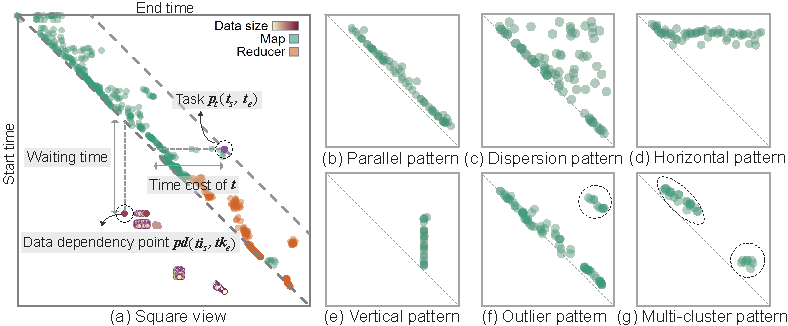
\includegraphics[width=0.48\textwidth]{figures/visualization/distributionview_revision.pdf}
	\vspace{-2mm}
	\caption{\vtitle{Task view} and task time usage patterns}
	\label{fig:distribution}
	\vspace{-6mm}
\end{figure}

\stitle{Temporal distribution}
Existing tools (e.g., SparkUI~\cite{sparkui} and Inviso~\cite{inviso}) usually employ Gantt chart to visualize the tasks, which are limited for two reasons: (i) Gantt chart causes severe visual clutter when visualizing massive (e.g., thousands) tasks; (ii) it is difficult to compare the time usage of different tasks as Gantt chart lacks proper alignment. 

To tackle these limitations, we plot the tasks as points in a square view.
In particular, we use the x-axis of the square view to represent the task start time and the y-axis to represent the task end time, which makes task $t$ a point, i.e., $p_t(t_s, t_e)$, in the square view. 
\qm{This configuration of the axes aligns with the conventional reading patterns observed in humans when browsing websites.} 
We use green and orange colors to encode the tasks of map and reducer job, respectively.
As shown in \autoref{fig:distribution}(a), this scatter point view design has several properties:
first, all points are in the top-right half of the square view because $t_e > t_s$ holds for all tasks;
second, the horizontal distance between the diagonal line and point $p_t$ encodes the time usage of task $t$, as illustrated by the dashed line in \autoref{fig:distribution}(a).
For interactive analysis, when a user moves the mouse on a task $t$, we plot a gray dashed auxiliary line that is parallel to the diagonal line and passes through point $p_t$ to show the time usage of the task. \qm{More importantly, for all tasks of a job, the distribution patterns of the points in the scatter point view reveal the query execution status and provide useful hints for the root causes of execution problems.
Figures~\ref{fig:distribution}(b) to (g) show the most representative patterns we observed in the production environment. We provide our observed hints of them below. 
}

\squishlist
\item \sstitle{\textbf{Parallel} pattern in \autoref{fig:distribution}(b)} it suggests that all tasks have similar time usage, resulting in points that are parallel and close to the diagonal line. \qm{A dense and parallel pattern indicates the query is executed smoothly.}
\item \sstitle{\textbf{Dispersion} pattern in \autoref{fig:distribution}(c)} it means that the tasks of a job have different start time and end time.\qm{
It suggests that these tasks may encounter multiple problems at the same time, such as insufficient resources, load imbalances, and limited executors, etc.
}

\item \sstitle{\textbf{Horizontal} pattern in \autoref{fig:distribution}(d)} it means all tasks start at almost the same time but end at different times.\qm{
As a special case of Dispersion pattern, it indicates the number of containers is enough, since all tasks can be executed at the same time.
}
\item \sstitle{\textbf{Vertical} pattern in \autoref{fig:distribution}(e)} it shows that the tasks finish together.\qm{
The vertical pattern appears typically because these tasks are all waiting for input data from a same upstream task which is usually the bottleneck.
}
\item \sstitle{\textbf{Outlier} pattern in \autoref{fig:distribution}(f)} it reveals that several tasks have much longer time usage than others. \qm{It indicates that these tasks may suffer from data skewness or deadlock. These tasks are largely the bottleneck of the query execution.
}
\item \sstitle{\textbf{Multi-cluster} pattern in \autoref{fig:distribution}(g)} it shows several separated groups of tasks. \qm{It usually indicates the execution of the job is interrupted for a period of time, which is usually caused by hardware problems or inefficient resources.}
\squishend



\stitle{Alternative design}
Several design alternatives for \textit{distribution view} are considered, including the Gantt chart, Marey's chart and Arc chart, which have been used in related research work and software. 
\autoref{fig:alt} shows the implementation of these designs and our methods with the same dataset. The green and orange colors indicate Map and Reducer tasks, respectively. 
Gantt chart is the most intuitive design to visualize the tasks through rectangular bars, however, when data is large, the height of bars will become too narrow to be observed. The other two designs all use lines (curves) instead of bars to show the temporal information of tasks. Marey's chart uses two horizontal axes to indicate the start time and end time, thus the task can be represented as a line connecting the two axis. Arc chart uses arcs to show the tasks, with two end points of the arc indicating the start time and end time. 
All these designs work well when the data size is small. However, in our application, the number of tasks will reach tens of thousands, which results in different problems for each design. For instance, the height of bars becomes too narrow to observe in  Gantt chart; Marey's chart and Arc chart all have serious visual clutter results from the overlap and cross of lines (curves), especially for Marey's graph, the orange lines are too dense to reflect any patterns. 

\begin{figure}[t]
	\centering
	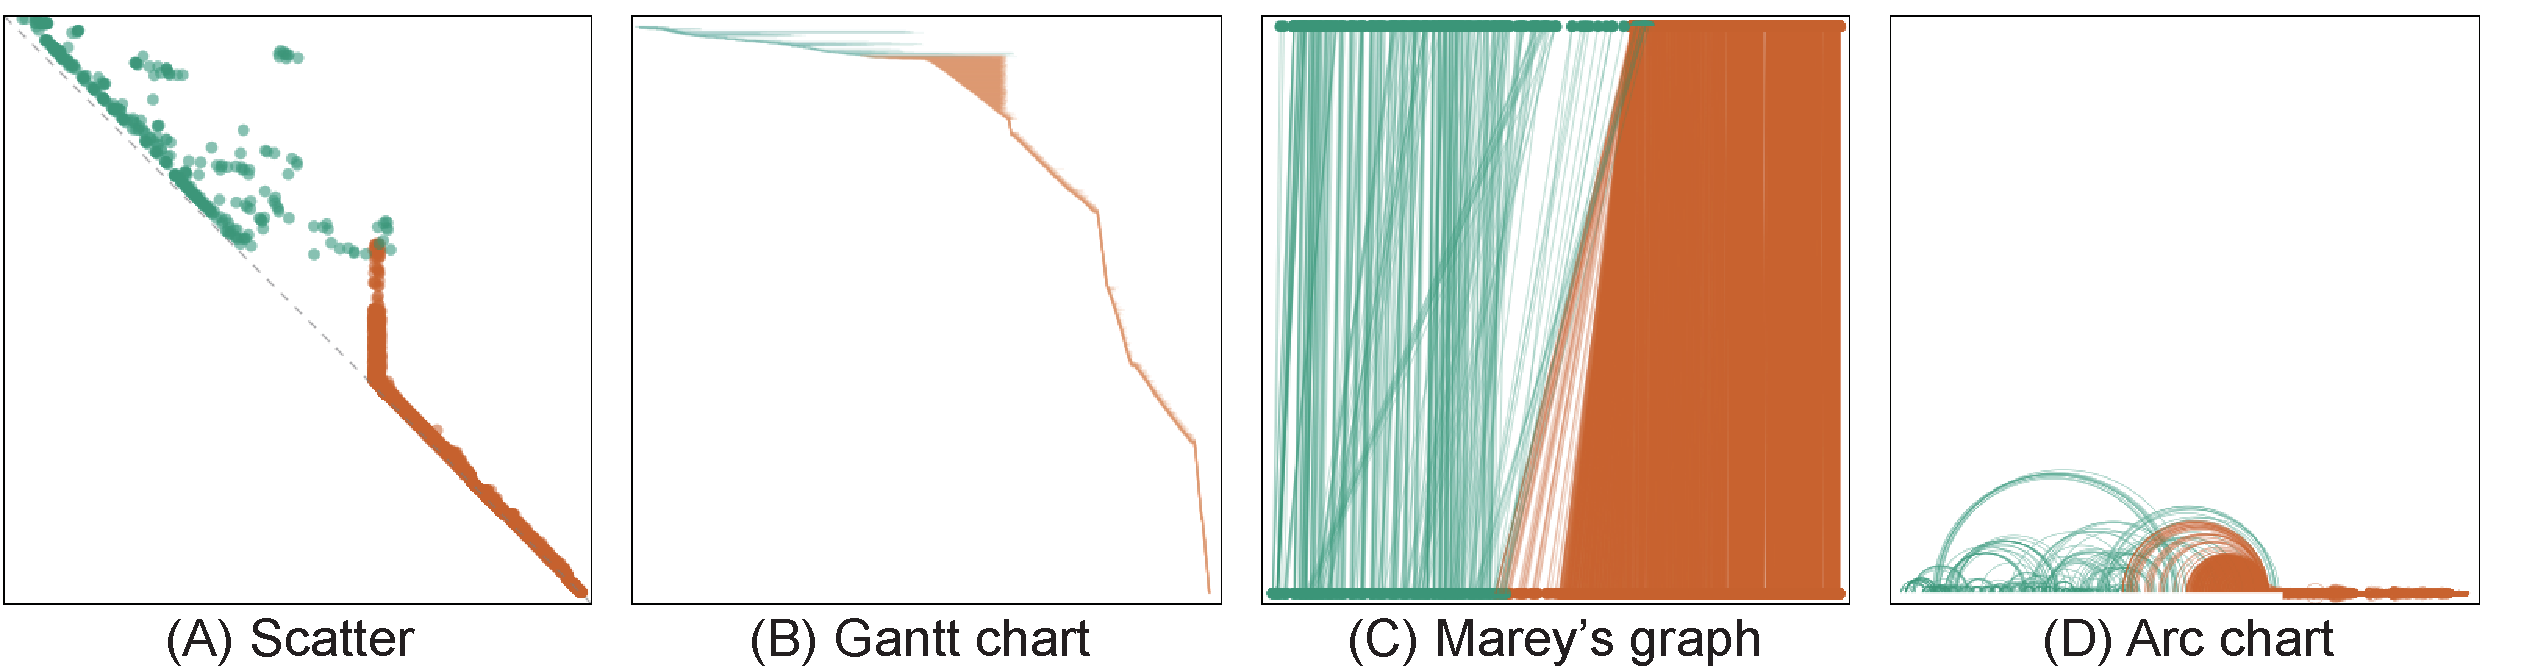
\includegraphics[width=0.48\textwidth]{figures/visualization/alternative_design.pdf}
	\vspace{-3mm}
	\caption{Alternative design of task/dependency distribution}
	\label{fig:alt}
	\vspace{-8mm}
\end{figure}


\stitle{Data dependency distribution}
Consider two tasks $ti$ and $tk$ with data dependency, and the output of $ti$ is used as input by $tk$.
The start time of $tk$ should be later than the end time of $ti$ in the idle case but the opposite may happen in abnormal cases (usually caused by the resource scheduler).
To visualize these abnormal cases, 
we show the data dependency of $ti$ and $tk$ by plotting point $p_d(tk_s, ti_e)$ in the square view. 
As $tk_s<ti_e$, all these abnormal tasks are in the bottom-left half of the square view, as shown by the purple points in \autoref{fig:distribution}(a). Thus, the dependency distribution does not interfere with the temporal distribution, which is in the top-right half.     
We provide several interaction mechanisms in task distribution. For example, once a task is selected, its dependencies, upstream tasks and downstream tasks will be highlighted in red and blue colors, respectively. 
%Interactions such as semantic zoom and drag are supported to locate the details of interests.  

\subsubsection{Auxiliary views and interaction designs}\label{sec:other}
We provide a suite of auxiliary views and rich cross-view interactions in \qevis{} to help users explore query execution progress. Due to space limitation, we only present two auxiliary views (i.e., \vtitle{entity list} and \vtitle{profiling view}) and refer the interested readers to our GitHub repository for the other views (e.g., \vtitle{query list} in \autoref{fig:teaser}(a)).

\sstitle{Entity list} it shows detailed statistics of each job row by row, shown in \autoref{fig:teaser}(e). 
Users can click on the triangle at the leftmost side of each job (i.e., job level) to enter the machine level. 
By clicking the triangle at the machine level, all tasks executed by the machine will be listed. 
To visualize the features of tasks, we implement two visualization forms, i.e., rug plot~\cite{rug_plot} and Gantt chart, that will be selected automatically based on the features of interest.
Besides time usage, \vtitle{entity list} also allows users to select other features of interest (e.g., read/write data size) through the dropdown at the top of this view.


\sstitle{Profiling view} it is embedded into each panel in the \vtitle{task view} and consists of a suite of visualizations to show execution statistics such as task parallelism and system hardware usages as illustrated in \autoref{fig:teaser}(f).
For single variate features such as task parallelism and memory usage, we use the line chart, which can show the temporal change of the value. 
For multiple variate features such as CPU usage and Disk IO, we use a heatmap, which is widely used to visualize multiple values.


\stitle{The design of interactions}
\qevis{} supports flexible interactions and cross-view linkage to facilitate multi-view exploration. 
For example, when the user hovers the mouse on a job in the \vtitle{job view}, shown as the purple boundary in \autoref{fig:teaser}(b), all tasks of this job will be highlighted in the \vtitle{task view}, as purple points in \autoref{fig:teaser}(d). 
Conversely, if the user hovers the mouse on a task point in the \vtitle{task view}, the corresponding job in the \vtitle{job view} and \vtitle{entity list} will be highlighted. 
Moreover, when the user clicks on points in the \vtitle{task view}, the \vtitle{entity list} will be expanded to show the corresponding tasks and execution machines, shown as the purple items in \autoref{fig:teaser}(e). 
When the user puts the mouse on an element for more than three seconds, a widget showing detailed information about the element will be displayed. 
Shown as \autoref{fig:teaser}(d2), when we put the mouse on the purple task, the task information such as data read, records processed, and time costs of each phase are displayed. 






